\documentclass{article}
\usepackage[utf8]{inputenc}
\usepackage{graphicx}

\title{CHAPTER 3}
\author{Dian Markuci (1184095)}
\date{8 November 2019}

\begin{document}

\maketitle

\section{TEORI}
\subsection{Fungsi}\\
\item Fungsi merupakan satu blok program yang terdiri dari nama fungsi, input variabel dan variabel kembalian. Nama fungsi diawali dengan \textit{def} dan setelahnya tanda titik dua. Nama bisa sama dan isinya berbeda apabila menggunakan huruf besar dan kecil atau case sensitive.\\

\item  Contoh dari fungsi sederhana:
\begin{center}
    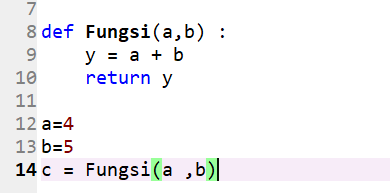
\includegraphics[width=8cm\textwidth]{figure/fungsi1.png}
\end{center}

\subsection{Package}
\item sebuah folder yang menyimpan source code
\item Cara pemanggilan :
 misal ditempat penyimpanan main program saya membuat sebuah folder buku dan dalamnya kita membuat sebuah source code dengan nama literasi.py, cara pemanggilannya yaitu sebagai berikut :
 
 \begin{center}
     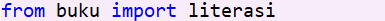
\includegraphics[width=8cm\textwidth]{figure/package.png}
 \end{center}

\subsection{Kelas, Objek, Atribut, Method}
\item Kelas merupakan sebuah blueprint dari sebuah objek 
\item  Objek merupakan perwujudan dari sebuah class.
\item  Atribut merupakan semua class yang membuat objek dan semua objek tersebut mengandung karakteristik.
\item method merupakan fungsi yang didefinisi dalam suatu class.

\subsection{Pemanggilan library kelas dari instansiasi dan pemakaiannya contoh dengan program}

\begin{center}
    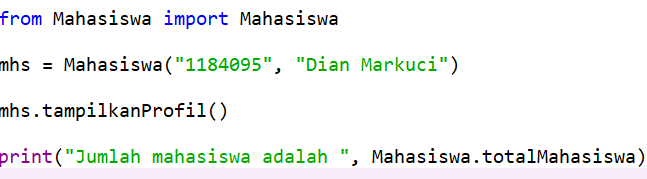
\includegraphics[width=10cm\textwidth]{figure/manggil.png}
\end{center}

\subsection{Pemakaian paket dengan from kalkulator import penambahan}

\begin{center}
    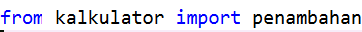
\includegraphics[width=8cm\textwidth]{figure/kalkk.png}
\end{center}
memanggil package lalu tambahkan kode penambahan #bisa dibaca dengan import penambahan dari folder kalkulator 

contoh:
\begin{center}
    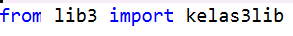
\includegraphics[width=6cm\textwidth]{figure/kalk.png}
\end{center}

\subsection{Paket fungsi file library ada di dalam folder}
\begin{center}
    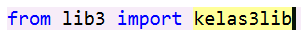
\includegraphics[width=6cm\textwidth]{figure/folder.png}
\end{center}
Jadi tulis dulu nama foldernya baru tulis import library nya\\


\section{Keterampilan Pemrograman}
\textit{soal 1}
\begin{center}
    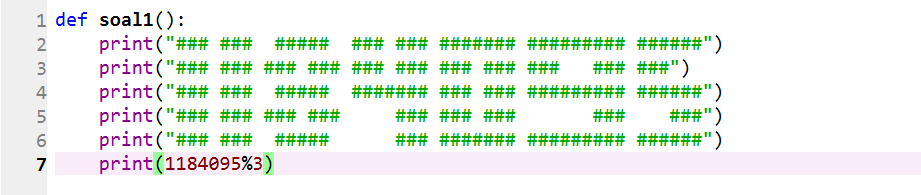
\includegraphics[width=15cm\textwidth]{figure/1.png}
\end{center}

\textit{soal 2}
\begin{center}
    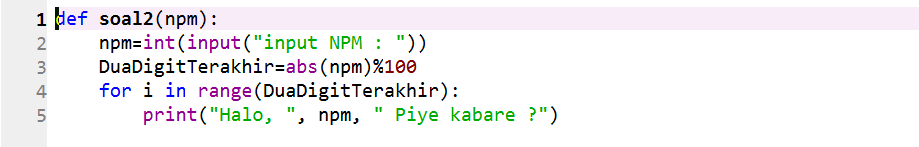
\includegraphics[width=15cm\textwidth]{figure/2.png}
\end{center}

\textit{soal 3}
\begin{center}
    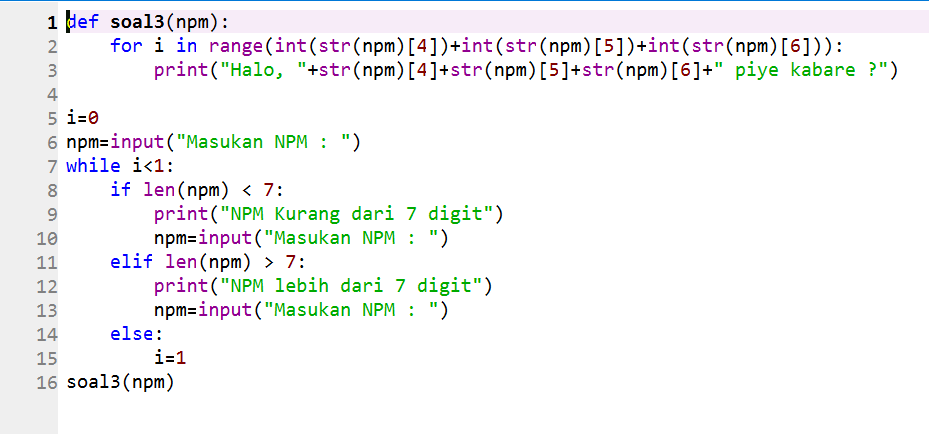
\includegraphics[width=15cm\textwidth]{figure/3.png}
\end{center}

\textit{soal 4}
\begin{center}
    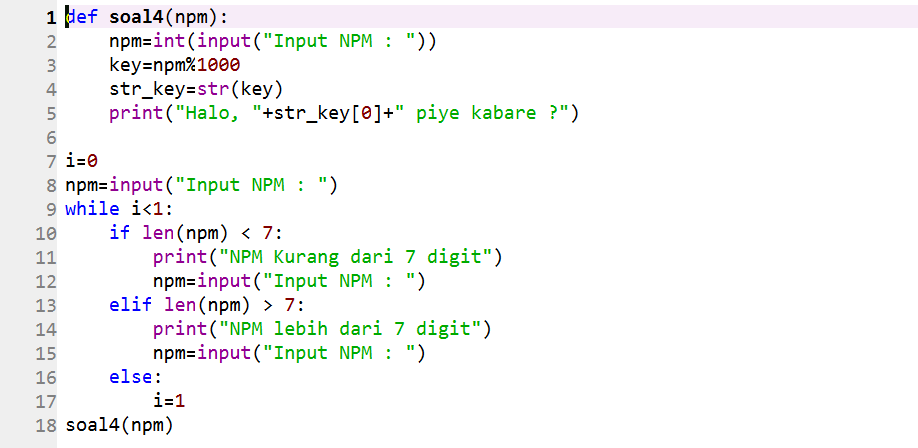
\includegraphics[width=15cm\textwidth]{figure/4.png}
\end{center}

\textit{soal 5}
\begin{center}
    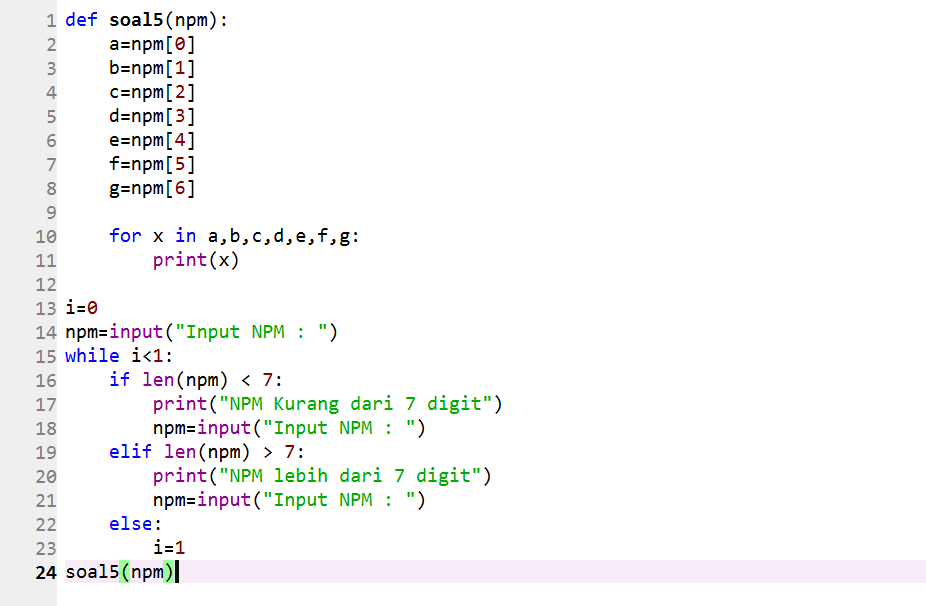
\includegraphics[width=15cm\textwidth]{figure/5.png}
\end{center}

\textit{soal 6}
\begin{center}
    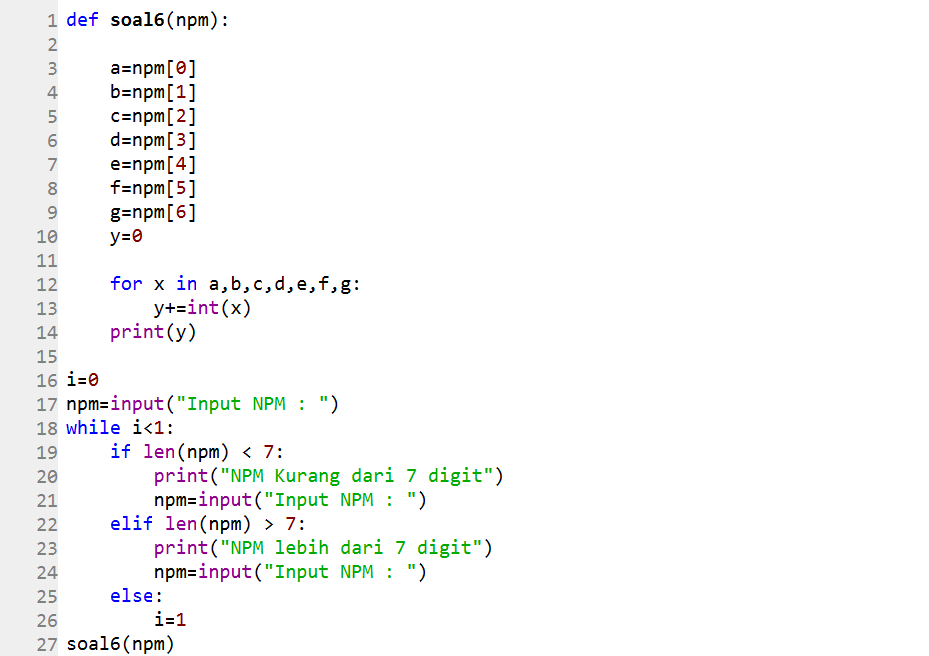
\includegraphics[width=15cm\textwidth]{figure/6.png}
\end{center}

\textit{soal 7}
\begin{center}
    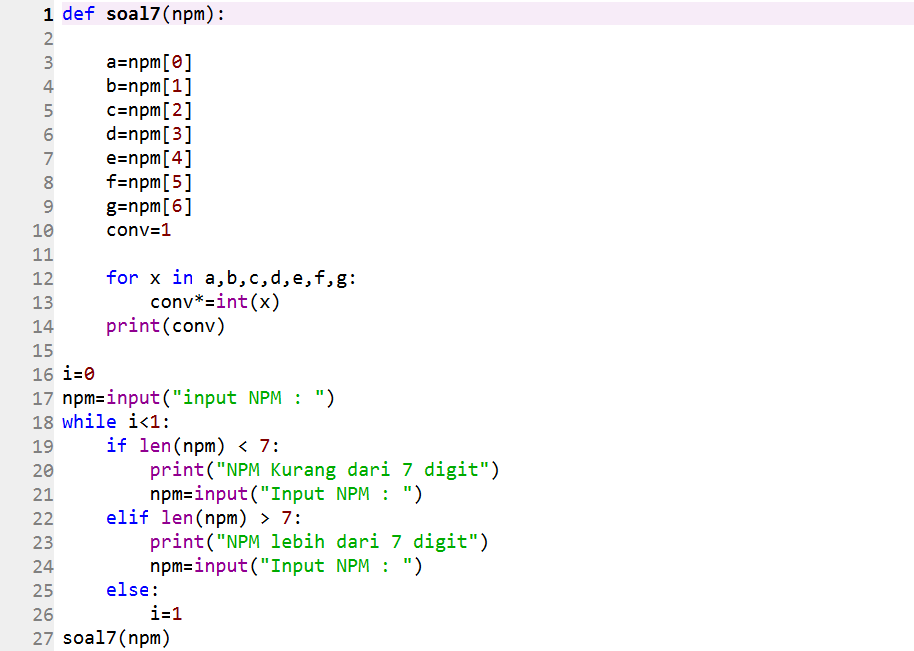
\includegraphics[width=15cm\textwidth]{figure/7.png}
\end{center}

\textit{soal 8}
\begin{center}
    
\includegraphics[width=15cm\textwidth]{figure/8.png}
\end{center}

\textit{soal 9}
\begin{center}
    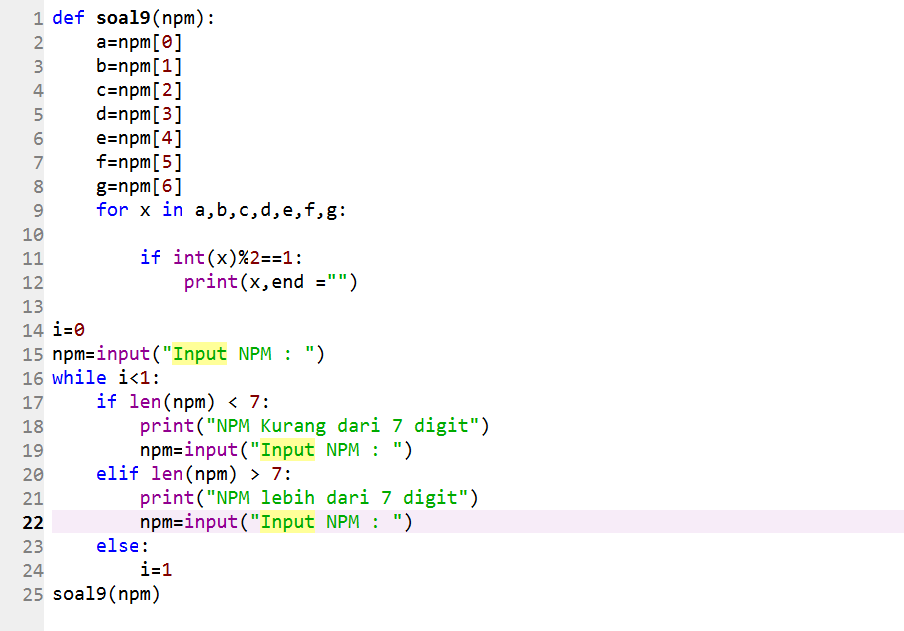
\includegraphics[width=15cm\textwidth]{figure/9.png}
\end{center}

\textit{soal 10}
\begin{center}
    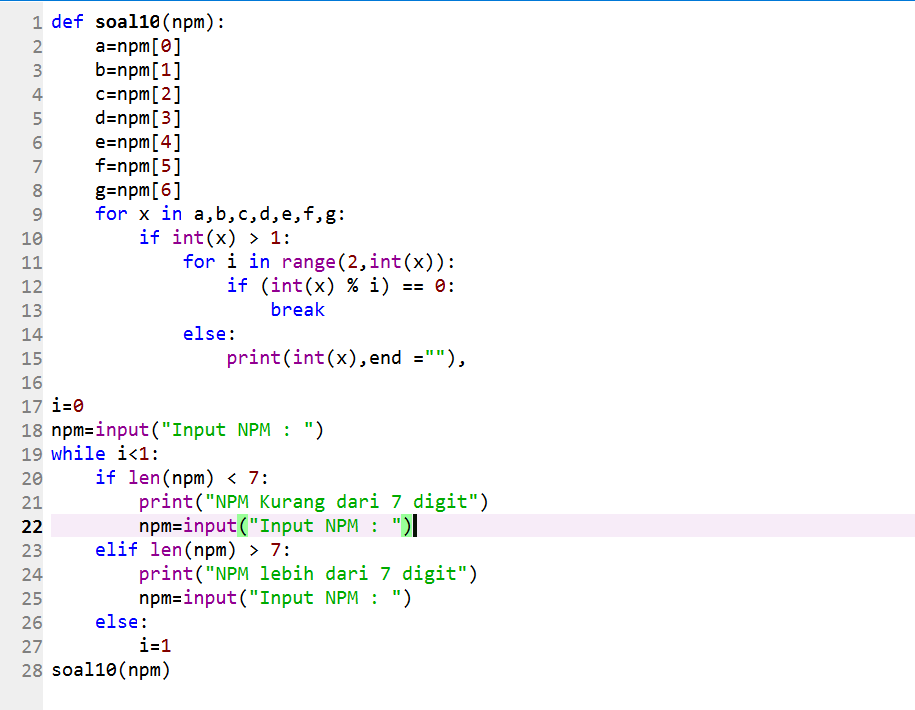
\includegraphics[width=15cm\textwidth]{figure/10.png}
\end{center}

\end{document}
